%\documentclass[iop]{emulateapj}
\documentclass[aps, pre, onecolumn, nofootinbib, notitlepage, groupedaddress, amsfonts, amssymb, amsmath, longbibliography]{revtex4-1}
\usepackage{tabularx}
\usepackage{graphicx}
\usepackage{hyperref}
\usepackage{xcolor}
\hypersetup{
    colorlinks,
    linkcolor={red!50!black},
    citecolor={blue!50!black},
    urlcolor={blue!80!black}
}
\usepackage{bm}
\usepackage{natbib}
\usepackage{longtable}
\LTcapwidth=0.87\textwidth

\newcommand{\Div}[1]{\ensuremath{\nabla\cdot\left( #1\right)}}
\newcommand{\DivU}{\ensuremath{\nabla\cdot\bm{u}}}
\newcommand{\angles}[1]{\ensuremath{\left\langle #1 \right\rangle}}
\newcommand{\grad}{\ensuremath{\nabla}}
\newcommand{\RB}{Rayleigh-B\'{e}nard }
\newcommand{\stressT}{\ensuremath{\bm{\bar{\bar{\Pi}}}}}
\newcommand{\lilstressT}{\ensuremath{\bm{\bar{\bar{\sigma}}}}}
\newcommand{\nrho}{\ensuremath{n_{\rho}}}
\newcommand{\approptoinn}[2]{\mathrel{\vcenter{
	\offinterlineskip\halign{\hfil$##$\cr
	#1\propto\cr\noalign{\kern2pt}#1\sim\cr\noalign{\kern-2pt}}}}}

\newcommand{\appropto}{\mathpalette\approptoinn\relax}

\newcommand\mnras{{MNRAS}}%

\begin{document}
\author{Evan H. Anders}
\affiliation{Dept. Astrophysical \& Planetary Sciences, University of Colorado -- Boulder, Boulder, CO 80309, USA}
\affiliation{Laboratory for Atmospheric and Space Physics, Boulder, CO 80303, USA}
\author{Benjamin P. Brown}
\affiliation{Dept. Astrophysical \& Planetary Sciences, University of Colorado -- Boulder, Boulder, CO 80309, USA}
\affiliation{Laboratory for Atmospheric and Space Physics, Boulder, CO 80303, USA}
\author{Jeffrey S. Oishi}
\affiliation{Department of Physics and Astronomy, Bates College, Lewiston, ME 04240, USA}
\title{Accelerated convergence of convective simulations using boundary value problems}

\begin{abstract}
We present a method for coupling boundary value problems (BVPs) with initial value problems (IVPs)
in order to achieve thermally converged convective solutions on dynamical timescales, rather than the
long thermal timescale. We study this method in the context of \RB convection. 
We demonstrate that the solution reached by BVP and the
solution reached by a long thermal rundown of the IVP are similar, and demonstrate that this method works at a
large range of supercriticalities.  The BVP method is used to achieve converged solutions at high supercriticality ($10^8$),
and its extensions to more complex scenarios are discussed.
\end{abstract}
\maketitle


\section{Introduction}
\label{sec:intro}
Natural convection occurs in the presence of disparate timescales which
prohibit numericists from studying realistic models of natural systems.  For example,
flows in the Sun's convection zone range from a Mach number (Ma) of order unity
near the solar surface to order $10^{-5}$ deep in the solar interior.
Explicit methods which are bound by the Courant-Friedrich-Lewy
(CFL) timestep limit must resolve the fastest motions (sound
waves and surface convection), resulting in timesteps which are prohibitively
small for studies of the deep, low-Ma motions. These systems are numerically
stiff. Even in the absence of the fast surface motions, the disparity between
the sound crossing time and the deep flows have made studies of low-Ma stellar
convection difficult. Traditionally, approximations such as
the anelastic approximation, in which sound waves are explicitly filtered out,
have been used to study low-Ma flows \cite{brown&all2010, featherstone&hindman2016}.
More recently, advanced numerical techniques which use implicit or mixed
implicit-explicit timestepping mechanisms have made it feasible to study
convection at low Mach numbers \cite{viallet&all2011, viallet&all2013, viallet&all2016, lecoanet&all2014,
anders&brown2017, bordwell&all2018}, and careful studies of deep convection which
would have been impossible a decade ago are now widely accessible.

While solutions to problem of disparate dynamical timescales have proven useful,
the difference between convective timescales and system relaxation timescales remains
a significant problem facing studies of convection. 
As modern simulations aim to model natural convection
by increasing into the high-Rayleigh-number (Ra) regime,
the thermal diffusion timescale on which the system relaxes grows with respect
to the dynamical timescale, which stays roughly constant across all Ra
\cite{anders&brown2017}.
Solar convection is, once again, a prime example of this phenomenon.
Dynamical timescales in the Solar convective zone are relatively short 
(10 min overturn at solar surface, one month solar
rotation rate) compared to the Kelvin-Helmholtz timescale of
$3 \cdot 10^7$ years \cite{stix2003}.  
Furthermore, as dynamical and diffusive timescales separate, 
simulations become more turbulent. More turbulent motions 
require finer grid meshes and smaller timesteps
to capture advective dynamics. Thus, the progression of simulations into the high-Ra
regime of natural convection is slowed by two simultaneous effects: timestepping
through a single convective overturn time becomes more computationally expensive
while the number of overturn times required for systems to reach thermal equilibration
grows.

The vast difference between convective and diffusive timescales has long plagued
numericists studying convection, and a plethora of approaches has been employed to
study thermally converged solutions. One popular method for accelerating the convergence
of high-Ra solutions is by ``Bootstrapping,'' or the process of using the flow
fields in a converged solution at lower Ra as initial conditions for a simulation at a higher
Ra.  This method has been used with great success \cite{johnston&doering2009, verzicco&camussi1997},
but it is not without its faults.  Bootstrapped solutions are succeptible to hysteresis
effects, in which large-scale convective structures present in the
low Ra solution imprint onto the dynamics of the new, high Ra solution. 
In moderate-Ra simulations, a commonly-used tactic is to use 
a simple model of the full convective state as initial conditions.  
For example, past studies have used a linear eigenvalue solve to set the initial
convective state \cite{hurlburt&all1984} or used an axisymmetric solution 
as initial conditions for convection in a 3D cylinder \cite{verzicco&camussi1997}. 
In certain systems, 
the approximate state of the evolved solution can be estimated, and there an
appropriate set of initial conditions can either be solved for analytically
\cite{couston&all2017} or by using knowledge of Mixing Length Theory or other convective
theories to adjust the initial profile towards the proper adiabatic state \cite{brandenburg&all2005}.

Despite the plethora of methods that have been used,
the most straightforward way to achieve a thermally converged solution
is to evolve a convective simulation through a thermal timescale. Some modern
studies do just that \cite{featherstone&hindman2016}, but it is becoming
increasingly difficult. Such evolution is
\emph{expensive}, and state-of-the-art simulations at the highest values of Ra
can only be reasonably run
for tens to hundreds of buoyancy times \cite{stevens&all2011}, much less the
thousands of buoyancy timescales required for thermal convergence.

In this work, we study a method of achieving accelerated evolution of a
convective simulation through adjusting the thermodynamic state using information 
from resolved, convective dynamics. We couple measurements of the (non-converged)
convective solution with knowledge about energy balances in the eventual solution
to self-consistently adjust the mean thermodynamic profile towards. 
While such a method has been used previously \cite{hurlburt&all1986}, 
we find no explanation in the current literature of the steps involved in employing
this method, nor any study into the accuracy of such a method.
In section \ref{sec:experiment}, we describe our convective simulations, our
numerical methods, and our method for achieving accelerated evolution. In
section \ref{sec:results}, we compare solutions reached through the accelerated evolution
method to those that have been evolved through a full diffusive timescale, and we
examine select simulations at very high Ra which have achieved accelerated evolution. Finally,
in section \ref{sec:discussion}, we discuss extensions of the methods presented
here to stratified, compressible systems.

\section{Experiment}
\label{sec:experiment}
We study incompressible \RB convection under the Oberbeck-Boussinesq approximation,
such that our fluid
has a constant kinematic viscosity ($\nu$), thermal diffusivity ($\kappa$), and coefficient
of thermal expansion ($\alpha$). The density of the fluid is a constant, $\rho_0$, except on the
term where the constant gravitational acceleration, $\bm{g} = - g\hat{z}$, acts in the vertical momentum equation, 
where $\rho = \rho_0(1  - \alpha T_1)$.  
Under these constraints, the equations of motion are \cite{spiegel&veronis1960}
\begin{gather}
\DivU = 0, 
	\label{eqn:incompressible}
\\
\frac{\partial \bm{u}}{\partial t} + \bm{u}\cdot\grad\bm{u} =
-\frac{1}{\rho_0}\grad P - g( 1 - \alpha T_1)\hat{z} + \nu\grad^2\bm{u}, 
	\label{eqn:dim_bouss_momentum}
\\
\frac{\partial T_1}{\partial t} + \bm{u}\cdot\grad(T_0 + T_1) = \kappa\grad^2 T_1,
	\label{eqn:dim_bouss_energy}
\end{gather}
where $\bm{u} = u\hat{x} + v\hat{y} + w\hat{z}$ is the velocity, 
$T = T_0 + T_1$ are the initial and fluctuating components of temperature, 
and $P$ is the pressure.
We non-dimensionalize these equations such that the dimensionless unit of
length is the layer height ($L_z$),
temperature is in units of the initial temperature jump across the layer ($\Delta T_0 = L_z \grad T_0$), 
and velocity is in units of the freefall velocity ($v_{\text{ff}} = \sqrt{\alpha g L_z^2 \grad T_0}$).
by these choices, one time unit is a freefall time ($L_z/v_{ff}$).
We introduce a reduced kinematic pressure,
$\varpi \equiv P / \rho_0 + \phi + |\bm{u}|^2 / 2$, where the gravitational
potential, $\phi$, is defined such that $\bm{g} = -\grad \phi$. As $P$ is a
Langrange multiplier under the Oberbeck-Boussinesq approximation, $\varpi$
can be treated straightforwardly as a linear variable. 
In non-dimensional form, Eqns. \ref{eqn:dim_bouss_momentum} \& \ref{eqn:dim_bouss_energy}
are
\begin{gather}
\frac{\partial \bm{u}}{\partial t} + \grad \varpi - T_1\hat{z} + \mathcal{R}\grad\times\bm{\omega} = \bm{u}\times\bm{\omega}
	\label{eqn:bouss_momentum}
\\
\frac{\partial T_1}{\partial t} - \mathcal{P}\grad^2 T_1 + w \frac{\partial T_0}{\partial z} = - \bm{u}\cdot\grad T_1.
	\label{eqn:bouss_energy}
\end{gather}
where $\bm{\omega} = \grad \times \bm{u}$ is the vorticity.
The dimensionless control parameters $\mathcal{P}$ and $\mathcal{R}$ 
are set by the Rayleigh and Prandtl numbers,
\begin{equation}
\mathcal{R} \equiv \sqrt{\frac{\text{Pr}}{\text{Ra}}}, \qquad \mathcal{P} \equiv \frac{1}{\sqrt{\text{Pr}\,\text{Ra}}}, \qquad
\text{Ra} = \frac{g \alpha L_z^4 \grad T_0}{\nu\kappa} = \frac{(L_z\,v_{\text{ff}})^2}{\nu\kappa}, \qquad \text{Pr} = \frac{\nu}{\kappa}.
\end{equation}
We hold Pr$ = 1$ constant throughout this work, such that $\mathcal{P} = \mathcal{R}$.

We study 2D and 3D convection in which the domain is a cartesian box, 
whose dimensionless vertical extent is $z \in [-1/2, 1/2]$, 
and which is horizontally period with an extent of $x, y \in [0, \Gamma]$ where $\Gamma = 2$ is the aspect
ratio. 
In the 2D cases, we set $v = \partial_y = 0$.
We specify no-slip, impenetrable boundary conditions at both the top and
bottom boundary and we use mixed thermal boundary conditions, such that
\begin{equation}
u = v = w \, \, \text{at}\,\,z = \pm 1/2, \qquad T_1 = 0 \,\,\text{at}\,\, z=+1/2, \qquad
\frac{\partial T_1}{\partial z} = 0\,\,\text{at}\,\,z=-1/2.
\label{eqn:bcs}
\end{equation}
For this choice of boundary conditions, the critical value of Ra at which
the onset of convection occurs is Ra$_{\text{crit}} = 1295.78$, and the
supercriticality of a run is defined as $S \equiv \text{Ra}/\text{Ra}_{\text{crit}}$.
Studies of convection which aim to model
astrophysical systems such as stars often employ mixed thermal
boundary conditions \cite{hurlburt&all1984, cattaneo&all1991, korre&all2017},
as we do here; however, our choice of thermal boundary conditions here
reflects the fact that the conditions in Eqn. \ref{eqn:bcs} are the simplest
to implement in the process of accelerated evolution (see section \ref{subsection:ae})
we study here.

We utilize the 
Dedalus\footnote{\url{http://dedalus-project.org/}} 
pseudospectral framework \cite{burns&all2016} to evolve  
Eqns. (\ref{eqn:incompressible}), (\ref{eqn:bouss_momentum}), \& (\ref{eqn:bouss_energy}) 
forward in time
using an implicit-explicit (IMEX), third-order, four-step 
Runge-Kutta timestepping scheme RK443 \cite{ascher&all1997}.  
The linear terms (on the LHS of the equations) are solved implicitly,
while the nonlinear terms (RHS) are explicitly solved.
Variables are time-evolved on a dealiased Chebyshev (vertical)
and Fourier (horizontal, periodic) domain in which the
physical grid dimensions are 3/2 the size of the coefficient grid.  

As initial conditions, we fill $T_1$ with
random white noise whose magnitude is $10^{-6}\mathcal{P}$.
This ensures that the initial perturbations are much smaller than the
evolved convective temperature perturbations, even at large Ra.
We filter this noise spectrum in coefficient space, 
such that only the lower 25\% of the coefficients
have power.

\subsection{The method of accelerated evolution}
\label{subsection:ae}
Here we describe a method of Accelerated Evolution (AE). We use this method to quickly evolve the
thermodynamic state of our solutions.  We compare this method to Standard Evolution
(SE), in which we naively evolve the atmosphere for one thermal diffusion time,
$t_\kappa = \mathcal{P}^{-1}$. As Ra increases, SE solutions become intractable, 
while the timeframe of convergence for an AE solution remains nearly constant
(in units of freefall times).
For an example of time saving achieved by using AE, we compare
energy traces at $S = 10^5$ from a SE run in Fig \ref{fig:time_trace}a to an AE run
in Fig. \ref{fig:time_trace}b.

\begin{figure}[t]
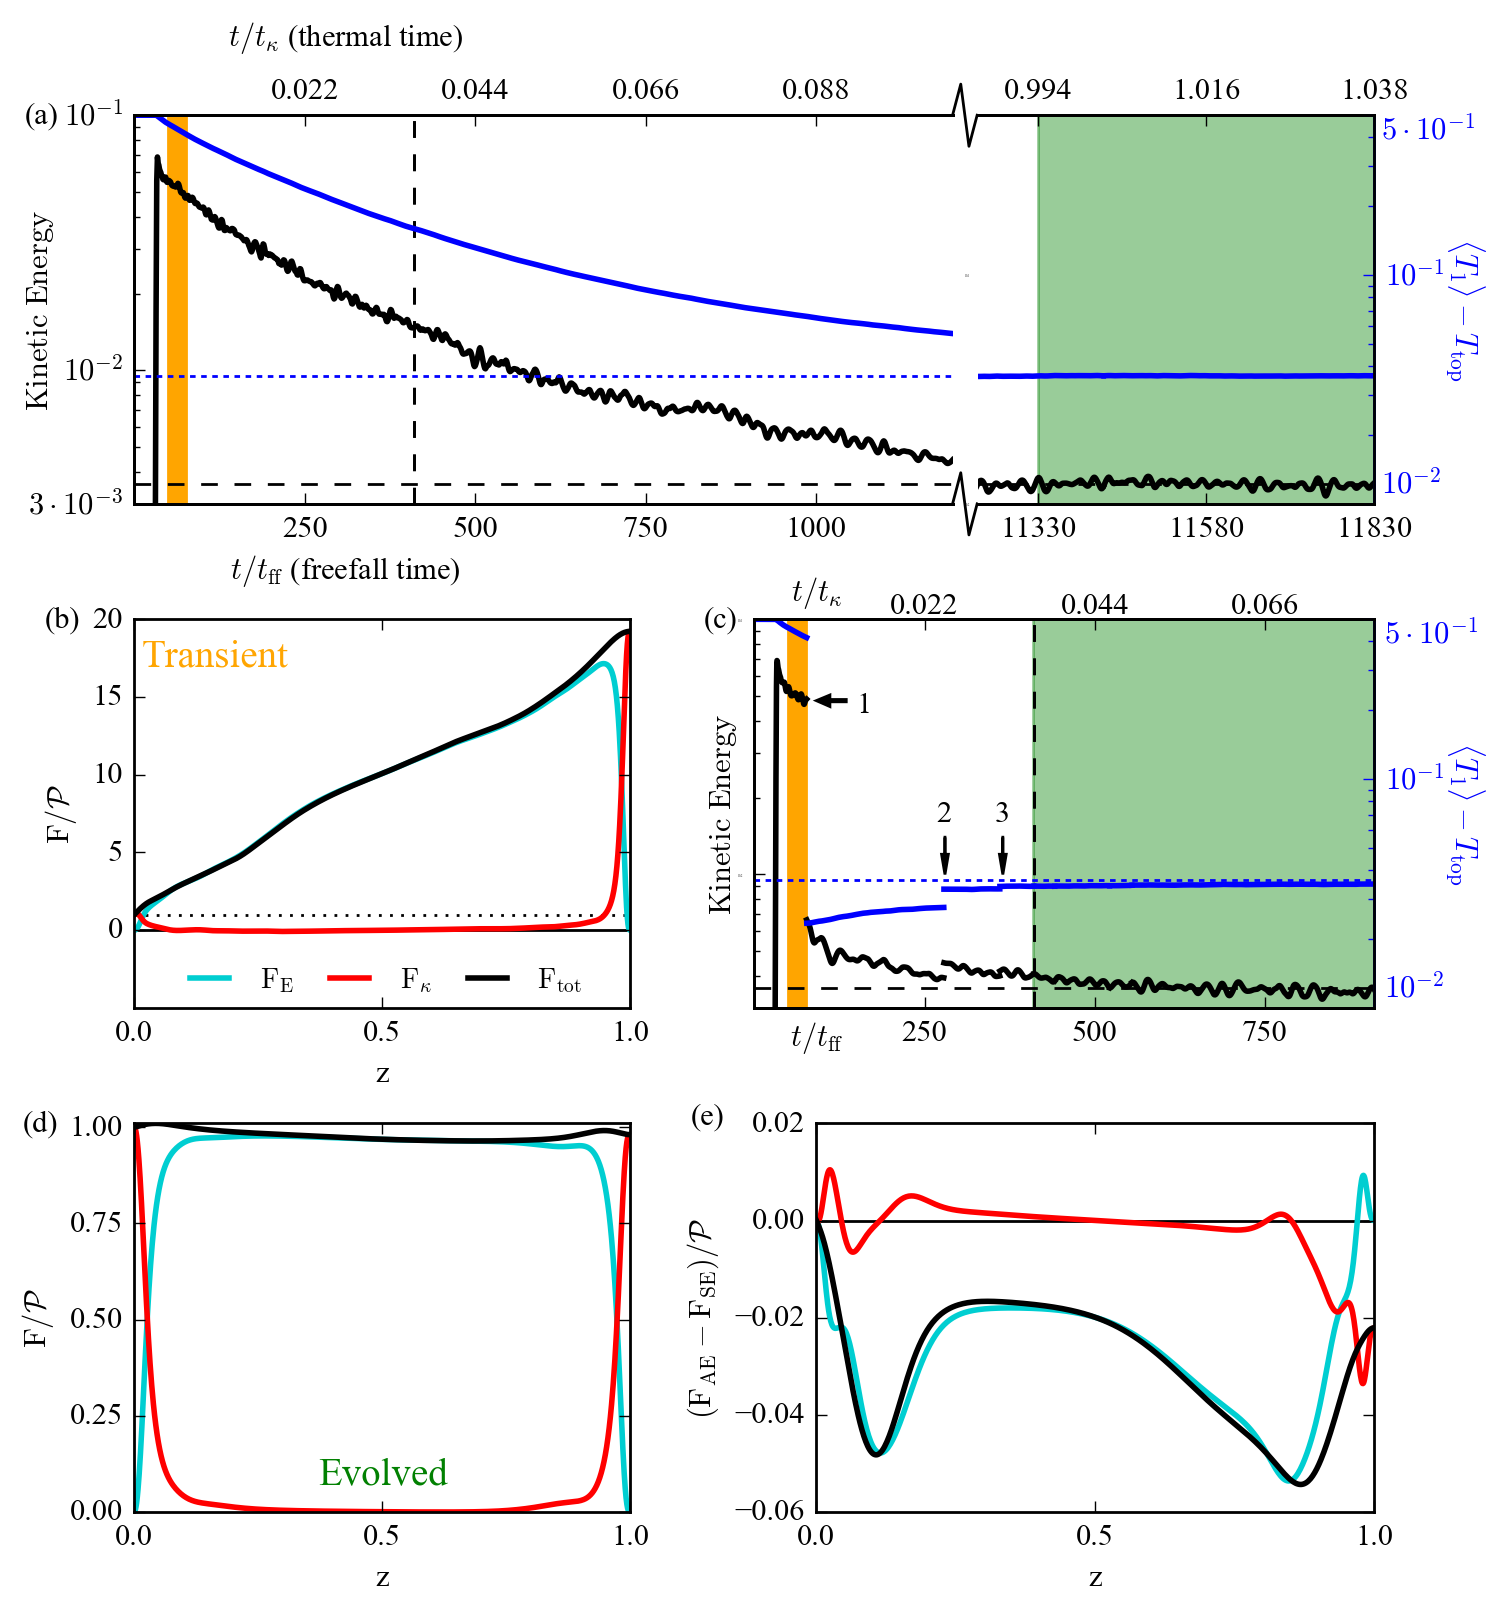
\includegraphics[width=\textwidth]{./figs/time_trace.png}
\caption{Traces of system energies vs. time for a long thermal rundown (a) and BVP convergence
(b) are shown for $S = 10^{4 + 2/3}$.  The horizontal extent of the subplots is set
such that one simulation time unit takes up an equal amount of paper space in (a) and (b). Volume averaged
kinetic energy is shown in black, and the volume averaged temperature with the top value removed, is shown
in red.
The dashed vertical line on (a) represents the time at which averaging begins in the BVP solution in (b),
and the horizontal dashed lines show the equilibrium value of the energies. The blue vertical lines represent
the beginning of the time-averaging window.
(c) System fluxes early in the run (the orange highlights in (a)) are shown.  
Black is the sum of the flux, purple
is the convective flux, and red is the conductive flux.
(d) Fluxes in the converged rundown IVP compared to the converged BVP.  The sum of flux is shown in
black \& grey, the convective flux is shown in purple \& pink, and the conductive flux is shown in red \& orange.
(e) The differences between the BVP and rundown fluxes is shown.  While not in perfect agreement, 
the BVP fluxes deviate from the rundown fluxes by only a few percent of the total flux, and
are much closer to the converged state than the initial fluxes, as in (c).
\label{fig:time_trace} }
\end{figure}

The horizontally averaged profiles of the vertical conductive flux, 
F$_{\text{cond}} = \angles{-\kappa\grad(T_0 + T_1)}_{x,y}$, and the vertical convective flux,
F$_{\text{conv}} = \angles{w(T_0 + T_1)}_{x,y}$, are the basis of the AE method. We measure
both of these quantities early in a simulation, as in Fig. \ref{fig:time_trace}c.
At these early stages in the simulation, these flux profiles are highly asymmetric,
with much more flux leaving through the upper boundary than entering through the
lowe boundary as the atmosphere approaches the proper isotherm selected by the
fixed temperature upper boundary.
However, by calculating the total flux,
F$_{\text{tot}} = $F$_{\text{conv}} +$ F$_{\text{cond}}$, and then calculating the profiles
\begin{equation}
f_{\text{conv}}(z) = \frac{F_{\text{conv}}}{F_{\text{tot}}},\qquad
f_{\text{cond}}(z) = \frac{F_{\text{cond}}}{F_{\text{tot}}},
\label{eqn:bvp_ratios}
\end{equation}
We presume that the early convection occupies roughly the same volume as the evolved
convection, and thus that the early thermal boundary layers are roughly the proper
width.  Where $f_{\text{conv}} = 1$, convection dominates all transport, and where
$F_{\text{cond}} = 1$, conduction dominates all transport (in the boundary
layers). Under this assumption, the proper evolved atmospheric flux profiles
are F$_{\text{conv, ev}} = \text{F}_{\text{bot}}\cdot f_{\text{conv}}$
and F$_{\text{cond, ev}} = \text{F}_{\text{bot}}\cdot f_{\text{cond}}$,
where F$_{\text{bot}} = \mathcal{P}$ is the amount of flux entering the
bottom of the atmosphere.

In the evolved, time-stationary state, the horizontal- and time-average of
Eqns. (\ref{eqn:bouss_momentum}) and (\ref{eqn:bouss_energy}), neglecting terms that
vanish due to symmetry, are
\begin{gather}
\frac{\partial}{\partial z}\angles{\varpi}_{x,y} - \angles{T_1}_{x,y}\hat{z} = \angles{\bm{u}\times\bm{\omega}}_{x,y},
	\label{eqn:bouss_BVP_momentum}
\\
\frac{\partial}{\partial z}\text{F}_{\text{conv, ev}} - \mathcal{P}\frac{\partial^2}{\partial z^2} \angles{T_1}_{x,y} = 0.
	\label{eqn:bouss_BVP_energy}
\end{gather}
Convective flows
are perturbations around a thermal profile defined by these equations in the proper evolved, 
statistically stationary state. Furthermore, under the specification of
F$_{\text{conv, ev}}$ and $\angles{\bm{u}\times\bm{\omega}}_{x,y}$,
\emph{the mean thermodynamic structure of the system} ($\angles{\varpi}_{x,y},\,\angles{T_1}_{x,y}$)
\emph{is fully specified}.

The AE method is thus simple: we construct F$_{\text{conv, ev}}$ as described above.
Then we calculate a profile, 
$\xi(z) = \text{F}_{\text{conv, ev}}/\text{F}_{\text{conv}}$, which is the amount that the
flux in the system needs to be reduced by, as a function of height.
We multiply the velocities
and the thermal fluctuations, $T - \angles{T}$, by $\sqrt{\xi}$, such that the product of all fluctuations
(which carry the convective flux) are diminished by a factor of $\xi$.  We solve
Eqns. (\ref{eqn:bouss_BVP_momentum}-\ref{eqn:bouss_BVP_energy}) with F$_{\text{conv, ev}}$
and $\xi\cdot\angles{\bm{u}\times\bm{\omega}}_{x,y}$ for the mean thermodynamic state,
and then continue evolving in time.  This adjustment of the mean profile and the
diminishing of velocities and fluctuations is the AE method, and it can generally
be applied tens of buoyancy times after the peak of convective transient.

\section{Results}
\label{sec:results}
We study evolved solutions achieved through the SE method from convective onset
up to $S = 10^5$ in 2D and $S = 10^4$ in 3D.  These SE runs are compared to
AE runs spanning from onset up to $S = 10^7$ in 2D and $S = 10^4$ in 3D.
For a full list of simulations, we refer the reader to appendix \ref{appendix:run_table}.

We report the time- and volume-averaged values of select measurements of the
evolved solutions in Fig. \ref{fig:parameter_space_comparison}.  We report
the scaling of heat transport in the evolved solution, as quantified by the
Nusselt number, in Fig. \ref{fig:parameter_space_comparison}a.
The volume averaged Nusselt number is defined as
\begin{equation}
\text{Nu} = \frac{\angles{F_{\text{conv}} + F_{\text{cond}}}}{\angles{F_{\text{cond, ref}}}}
 = \frac{\angles{wT - \mathcal{P}\partial_z T}}{\angles{- \mathcal{P} \partial_z T}}.
\end{equation}
In 3D and in 2D when $S < 10^{3+2/3}$, the evolved system is defined by a clear
value of Nu and the convection reaches a statistically stationary state.
In 2D and at larger values of $S$, the value of Nu oscillates as a function of time
as the plumes in the solution oscillate horizontally.  Our choice of no-slip
boundary conditions prevent the fluid from entering a full-fledged shearing state
\cite{goluskin&all2014}, but the oscillatory motions which do arise cause the
system to vary between periods of low heat transport and high heat transport.
The SE simulations which span up to $S = 10^5$ exhibit the same horizontally
oscillatory motion as the AE solutions for the same initial conditions. The
scaling of the mean value of Nu is roughly $\text{Nu} \propto \text{Ra}^{1/5}$,
weaker than that reported in similar systems with fixed-T and fixed-flux boundary
conditions \cite{johnston&doering2009}.  We attribute this weaker Nu scaling to
the oscillatory nature of the plumes, which may have been avoided by previous studies
using bootstrapping techniques as initial conditions.

In Fig. \ref{fig:parameter_space_comparison}b, we report the rms Reynolds number
in the AE solutions, where
$\text{Re} = \angles{|\bm{u}|} / \mathcal{R}$.  This measure scales roughly as
$\text{Re} \propto \text{Ra}^{0.45}$, and shows little variance with time.

In Fig. \ref{fig:parameter_space_comparison}c, we report the volume averaged 
temperature of the AE solutions, with the value at the upper (fixed $T$) boundary removed.
This measurement probes the thickness of the boundary layers of the solutions, and
should show scaling which is inversely proportional to Nu in converged solutions
where fixed-flux boundary conditions are used \cite{otero&all2002}.  We find here
that $(\angles{T} - T_{\text{top}}) \propto \text{Ra}^{-1/5}$, precisely the inverse
scaling of Nu, giving confidence that these solutions are in a converged state.

In Fig. \ref{fig:parameter_space_comparison}d-f, we report the fractional difference
between measurements from the AE solutions and measurements from the SE solutions.
We find that the mean value of Nu from AE solutions is accurate to the values
from SE solutions to within $\sim 1$\%, and the same is true for $\angles{T}$ measurements.
Re measurements show slightly greater error, with AE measurements being on average
$\leq 2$\% away from the SE measurements. 

\begin{figure}[t]
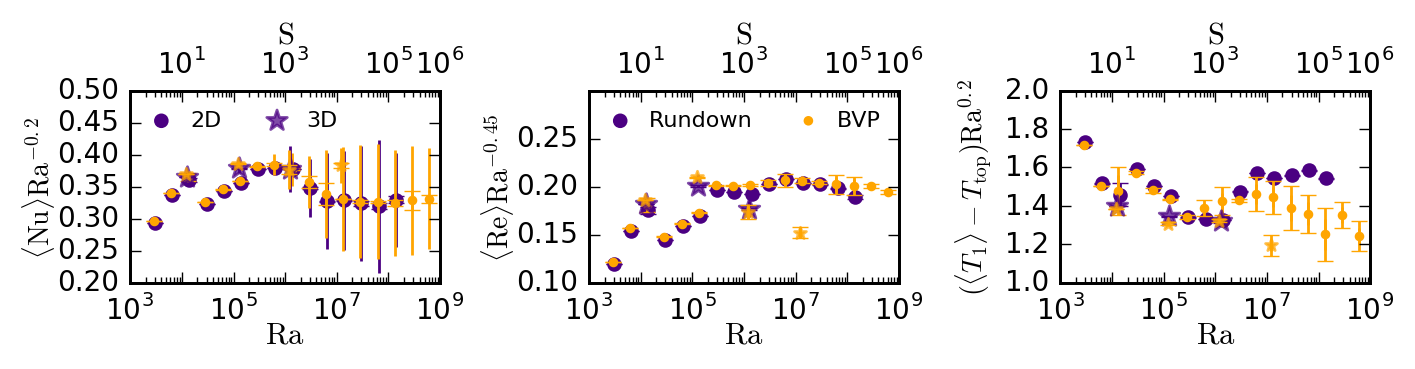
\includegraphics[width=\textwidth]{./figs/parameter_space_comparison.png}
\caption{Scaling plots are shown for the Nusselt number (a), the
Reynolds number (b), and the volume-averaged temperature (c).  
Symbols represent the mean value of
a measurement, vertical lines represent the standard deviation of the measurement over the
time window, and error bars represent the shift in the mean value over the window.
(a) Nu, which measures heat transport, scales roughly like $Ra^{1/5}$, and above Ra$\geq 10^6$,
simulations display horizontally oscillating plumes which have oscillating periods of high transport
and low transport.  The mean value is marginally diminished as a result, and the variance of Nu with time
is large. (b) Re, which measures the level of turbulence in the evolved solution, scales as
Ra$^{0.45}$ in 2D and is not distinctly different in 3D. (c) The average temperature flucutation, minus the top
temperature, which is a scalar measure of the final average thermodynamic state and should approach zero
in the limit of infinitely large Ra.
The temperature profile is slow to adjust, and differences between
BVP solutions and rundown solutions are quite easy to pick out in this measure. (d-f)
Relative error is shown between the BVP and IVP measurements of Nu (d), Re (e), and the
mean temperature (f). The grey box indicates the region in which only BVP runs were
carried out due to computational expense.
\label{fig:parameter_space_comparison} }
\end{figure}

The measurements presented in Fig. \ref{fig:parameter_space_comparison} demonstrate
that the AE method can be powerfully employed in parameter space studies in which
large numbers of simulations are compared in a volume-averaged sense.  We now turn
our examination to a more direct comparison of AE and SE for convection at
$S = 10^5$, as has been introduced in Fig. \ref{fig:time_trace}.

As the AE method primarily serves to adjust the thermodynamic structure of the
solution, we compare the temperature profile attained by AE and SE in 
Fig. \ref{fig:temp_comparison}.  We see that the boundary layer length scale is 
nearly identical in the AE and SE solution (Fig. \ref{fig:temp_comparison}a), but that
the mean temperature in the interior differs by about 0.5\% on average
(Fig. \ref{fig:temp_comparison}b). The probability distribution function of point-by-point
temperature values are compared in Fig. \ref{fig:temp_comparison}c.  We construct
this PDF by interpolating our temperature field onto a regular grid, determing the
frequency distribution of all $T$ values, and then properly normalizing such that
the integral of the PDF is unity.  In addition to the
difference in mode which can be seen in the mean vertical profile, the SE case
has a broader spread of temperature values.  This can likely be attributed to the
slight overstabilization of the temperature profile obtained by the AE method
(as can be seen in Fig. \ref{fig:time_trace}a\&b).  One means of comparing two
probability distributions to determine if they are drawn from the same underlying
sample is through the use of a Kolmogorov-Smirnov (KS) \cite{wall&jenkins2012}.
In general, a KS test must be conducted on independent, uncorrelated data, which
poorly describes the point-by-point values of flow in a fluid simulation. Thus,
we will merely use the KS statistic, the maximum difference
between the cumulative distribution functions (CDFs) of the two sample distributions,
as a numerical method of directly comparing the two PDFs.  For the distributions
shown in Fig. \ref{fig:temp_comparison}c,
we find a KS statistic of 0.113 near the modes, which is large, and implies that
these two distributions are different.




\begin{figure}[t]
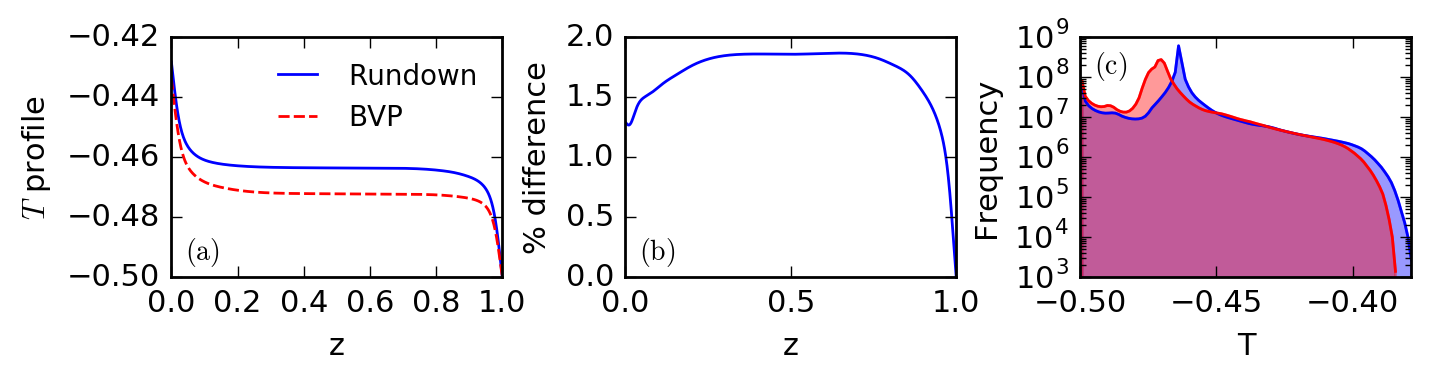
\includegraphics[width=\textwidth]{./figs/temp_comparison.png}
\caption{Comparisons of the evolved thermodynamic states of a BVP solution and a long IVP rundown at
$S = 10^{5}$ are shown.  (a) Evolved temperature profiles, as a function of height.
(b) The percentage difference between the temperature profiles (as shown in (a)), as a function of height.
(c) Probability distributions of point-by-point measurements of $T$ throughout the two domains over the
averaging windows are shown.  The cumulative distribution functions are overplotted and the maximum
difference between them in 0.0407. This difference arises due to the imperfect alignment of the
mean domain temperatures, but it is clear that otherwise the statistics are quite similar.
\label{fig:temp_comparison} }
\end{figure}

In addition to comparing the thermodynamic state achieved by the SE and AE methods,
we examine the velocities found in the evolved states.
We compute PDFs in the same manner as in Fig. \ref{fig:temp_comparison}c for the
vertical velocity (Fig. \ref{fig:pdf_comparison}a), horizontal velocity (Fig. \ref{fig:pdf_comparison}b),
and the nonlinear convective flux (Fig. \ref{fig:pdf_comparison}c). We report KS statistics
of 0.0577, 0.858, and 0.0347, respectively.  Perhaps unsurpisingly, the nonlinear
convective transport between the SE and AE methods are very similar, as is captured
in a volume-averaged sense in the Nu measurements of Fig. \ref{fig:parameter_space_comparison}a\&d).
In general, the velocity boundary conditions (Eqn. \ref{eqn:bcs}) more strongly dominate the flow
fields for the SE cases than the AE cases in Fig. \ref{fig:pdf_comparison}a\&c. 
This suggests that the velocity boundary layers are not yet fully formed in the
AE solutions. However, aside from this difference, the two solutions show a similar
distribution of realized velocity values.

\begin{figure}[b]
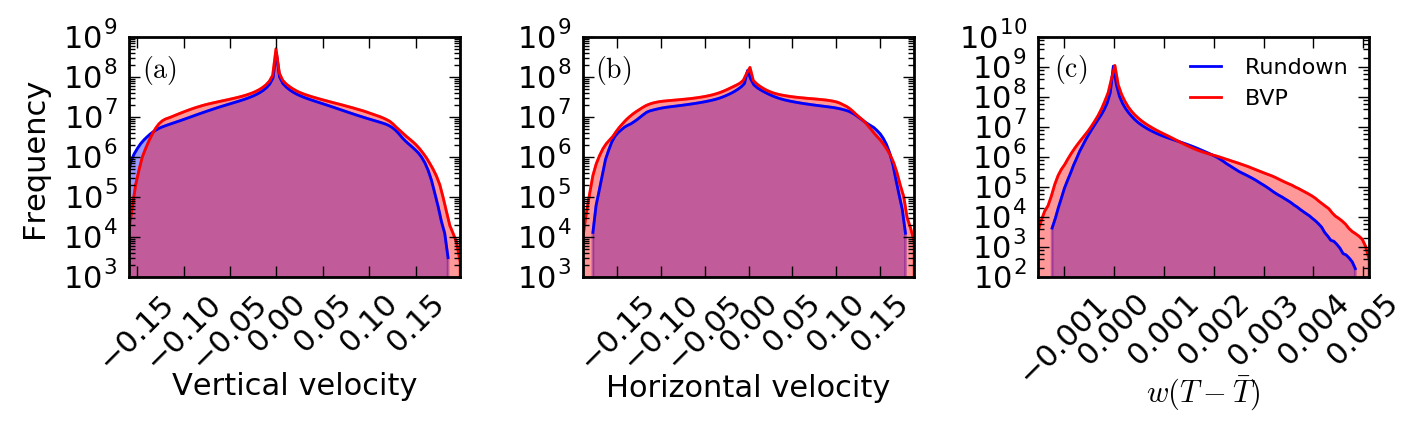
\includegraphics[width=\textwidth]{./figs/pdf_comparison.png}
\caption{Probability distribution functions of (a) the vertical velocity, (b) the horizontal velocity, and (c) nonlinear
convective transport are shown for a 2D runs achieved through the SE and AE methods
at $S = 10^{5}$.  Flows are sampled every 0.1 time units for 500 total time units,
and flows are interpolated onto an evenly spaced grid before sampling.
The cumulative distribution function is overplotted on each plot. 
\label{fig:pdf_comparison} }
\end{figure}


Despite differences between the SE and AE solutiosn for the case studied in 
Figs. \ref{fig:time_trace}, \ref{fig:temp_comparison}, \& \ref{fig:pdf_comparison},
the AE method is still extremely powerful.  The first application of the AE method
($t \approx 70$ in Fig. \ref{time_trace}b) immediately increases the 
average time step of our solver by a factor of 2-3. At higher supercriticality
($S = 10^7$), the AE solve immediately boosts the timestep by nearly a factor of 4.
Thus, not only does this method evolve the solution into nearly the correct state, 
but further time evolution (either to achieve precisely the correct thermodynamic
state or to take measurements of fluid quantities) happens more efficiently.


\section{Discussion \& Conclusions}
\label{sec:discussion}
The method presented here is a first step towards taking meaningful measurements
of highly turbulent convection on manageable, human timescales.  As demonstrated in Figs.
1-4, this BVP method quickly converges simulations to within a few percent of the true final
state. Furthermore, the total simulation time required to use the BVPs does not change drastically from
low $S$ to high $S$, so the main prohibition on high Ra states is the difficulty of timesteps becoming
increasingly small as turbulence increases.  Additionally, post-BVP, we generally see an increase of the
timestep size by nearly a factor of two due to the less intense driving of the near-converged state that
is achieved quickly.  

It is important to note that the measurements made in
this paper were generally done for short timescales (a few hundred buoyancy times) in
order to show the precise differences between the BVP solutions and the IVP solutions.
Where there are differences, the BVP solution is trending towards the IVP solution,
and if measurements were taken over long timescales (e.g., a thermal time), the
differences between the BVP solution and IVP solution would be negligible.

One major benefit of the BVP method used here is that it preserves the natural behavior of 
the convective solution (such as the horizontally oscillatory rolls
of high-Ra 2D states in Fig. \ref{fig:parameter_space_comparison}).
One frequently used method of measuring dynamics in high-Ra simulations is that of bootstrapping,
in which the converged solution of a low-Ra state is used as initial conditions for a higher-Ra
simulation.  While this method is powerful, it can be influenced by hysteresis effects,
and the steady rolls achieved at low Ra can result in an artifically over-stable high-Ra
roll solution.  The BVP method we present here uses random noise initial conditions which allows the
convective solution to naturally choose the dynamics.

Another benefit of our BVP method is that it can be easily extended to more complicated
configurations.  For example, to use this method in simulations of stratified compressible convection,
one need only adapt the BVP equations to the appropriate equations of hydrostatic equilibrium
and thermal equilibrium obtained by averaging the fully compressible, ideal gas
steady state momentum and energy equations \cite{anders&brown2017, lecoanet&all2014}.
In compressible convection, where the density is allowed to change,
it is also essential to conserve mass by adding boundary conditions on the integrated mas density at
the upper and lower boundaries, much as stellar structure codes do \cite{paxton&all2011}.

While we have not chosen to use them here, this BVP method can be extended to other boundary conditions.  
To solve for fixed temperature boundary conditions, the 
main difficulty is in finding the amount of flux through the system, $F_{\text{tot, steady}}$.
However, by knowing the averaged value of the conductive flux (from the boundary conditions)
and the ratios in Eqn. (\ref{eqn:bvp_ratios}), $F_{\text{tot, steady}}$ can be found.
In the case of
fixed flux boundary conditions, the temperature solution is degenerate.
However, using knowledge about the system -- such as the initial symmetry of the
RB state around $T = 0$, the final solution can be pegged onto the proper profile.

Future work will aim to apply the methods presented here to compressible systems,
internally heated systems, and systems with more complex forms of the conductive flux.


\begin{acknowledgments}
EHA acknowledges the support of the University of Colorado's George 
Ellery Hale Graduate Student Fellowship.
This work was additionally supported by  NASA LWS grant number NNX16AC92G.  
Computations were conducted 
with support by the NASA High End Computing (HEC) Program through the NASA 
Advanced Supercomputing (NAS) Division at Ames Research Center on Pleiades
with allocations GID s1647 and GID g26133.
\end{acknowledgments}


\appendix
\section{Table of Runs}
\label{appendix:run_table}
\begin{center}
\begin{tabularx}{\textwidth}{ X X X X X X X X X}
\hline															
$S$	&	Ra	&	nz	&	nx, ny	&	$t_{\text{therm}}$	&	$t_{\text{avg}}$	&	Nu$_{\text{rundown}}$	&	Nu$_{\text{BVP}}$	\\
\hline															
$10^{1/3}$	&	$2.79 \cdot 10^3$	&	32	&	128	&	$52.8$	&	100	&	(TBD)	&	(TBD)	\\
$10^{2/3}$	&	$6.01 \cdot 10^3$	&	32	&	128	&	$77.6$	&	100	&	--	&	--	\\
$10^1$	&	$1.30 \cdot 10^4$	&	32	&	128	&	$114$	&	100	&	--	&	--	\\
$10^{1 + 1/3}$	&	$2.79 \cdot 10^4$	&	32	&	128	&	$167$	&	100	&	--	&	--	\\
$10^{1 + 2/3}$	&	$6.01 \cdot 10^4$	&	32	&	128	&	$245$	&	100	&	--	&	--	\\
$10^2$	&	$1.30 \cdot 10^5$	&	64	&	256	&	$360$	&	100	&	--	&	--	\\
$10^{2 + 1/3}$	&	$2.79 \cdot 10^5$	&	64	&	256	&	$528$	&	100	&	--	&	--	\\
$10^{2 + 2/3}$	&	$6.01 \cdot 10^5$	&	64	&	256	&	$776$	&	100	&	--	&	--	\\
$10^3$	&	$1.30 \cdot 10^6$	&	128	&	512	&	$1.14 \cdot 10^3$	&	200	&	--	&	--	\\
$10^{3 + 1/3}$	&	$2.79 \cdot 10^6$	&	128	&	512	&	$1.67 \cdot 10^3$	&	500	&	--	&	--	\\
$10^{3 + 2/3}$	&	$6.01 \cdot 10^6$	&	256	&	1024	&	$2.45 \cdot 10^3$	&	500	&	--	&	--	\\
$10^4$	&	$1.30 \cdot 10^7$	&	256	&	1024	&	$3.60 \cdot 10^3$	&	500	&	--	&	--	\\
$10^{4 + 1/3}$	&	$2.79 \cdot 10^7$	&	256	&	1024	&	$5.28 \cdot 10^3$	&	500	&	--	&	--	\\
$10^{4 + 2/3}$	&	$6.01 \cdot 10^7$	&	256	&	1024	&	$7.76 \cdot 10^3$	&	500	&	--	&	--	\\
$10^5$	&	$1.30 \cdot 10^8$	&	512	&	2048	&	$1.14 \cdot 10^4$	&	500	&	--	&	--	\\
$10^{5 + 1/3}$	&	$2.79 \cdot 10^8$	&	512	&	2048	&	$1.67 \cdot 10^4$	&	500	&	--	&	--	\\
$10^{5 + 2/3}$	&	$6.01 \cdot 10^8$	&	512	&	2048	&	$2.45 \cdot 10^4$	&	500	&	--	&	--	\\
$10^6$	&	$1.30 \cdot 10^9$	&	1024	&	4096	&	$3.60 \cdot 10^4$	&	500	&	--	&	--	\\
\hline															
\end{tabularx}
\end{center}



\section{Accelerated Evolution Recipe}
\label{appendix:recipe}
In general, the BVP solve is completed in the following steps:
\begin{enumerate}
\item Run the convective IVP. Once the convection achieves a volume-averaged Re of $\sqrt{\text{Ra}/\text{Ra}_{\text{crit}}}$,
wait for 50 freefall time units.  
\item Start taking the averages of $F_{\text{conv}}$, $F_{\text{tot}}$, and $\angles{\bm{u} \times \bm{\omega}}$, waiting either
30 freefall time units or until the average profiles change by no more than 1 part in 1000 on a
given timestep, whichever is a more difficult criterion. This ensures that
the profiles being used in the BVP are steady and smooth, and that they sample the full behavior of the convection.
\item Construct $\angles{w T_1}_{\text{steady}}$, $\xi$, and $\angles{\bm{u}\times\bm{\omega}}_{\text{steady}}$
from the flux profiles.
\item Solve for $\angles{T_1}$ and \angles{\varpi} of the
evolved state.  Adjust the mean profiles in the IVP.
\item Multiply the velocity field and the fluctuations in $T_1$ about its horizontal average by $\sqrt{\xi}$ in the IVP. 
\item Continue running the IVP for freefall 50 time units to allow for the velocities to equilibrate to their new background state.
\item Repeat steps 2-6 to complete a second BVP and get closer to the right solution now that we
are far from the very unstable transient period.
\item Take averages for the amount of time specified for the given run in Appendix \ref{section:appendix_table}.
\end{enumerate}




\bibliography{biblio.bib}
\end{document}
